In order to enable the annotation and subsequent searching for experiments and files the data stored on the server is complimented by a database of information.

Each file uploaded to or generated by \appName\ belongs to an experiment which is identified by the experiment ID (expID). Each experiment created by the end user results in an entry in the database's \term{Experiment} table.

Each experiment contains files that were either generated during the experiment (\term{raw} data) or processed from these files (\term{profile} or \term{region} data).

The full database schema is shown in \refer{fig:dat_databaseSchema}. The tables and columns currently not utilized by \appName\ are in grey. These have not been removed from the database under expectation of future development.

\begin{figure}[p]
\centering
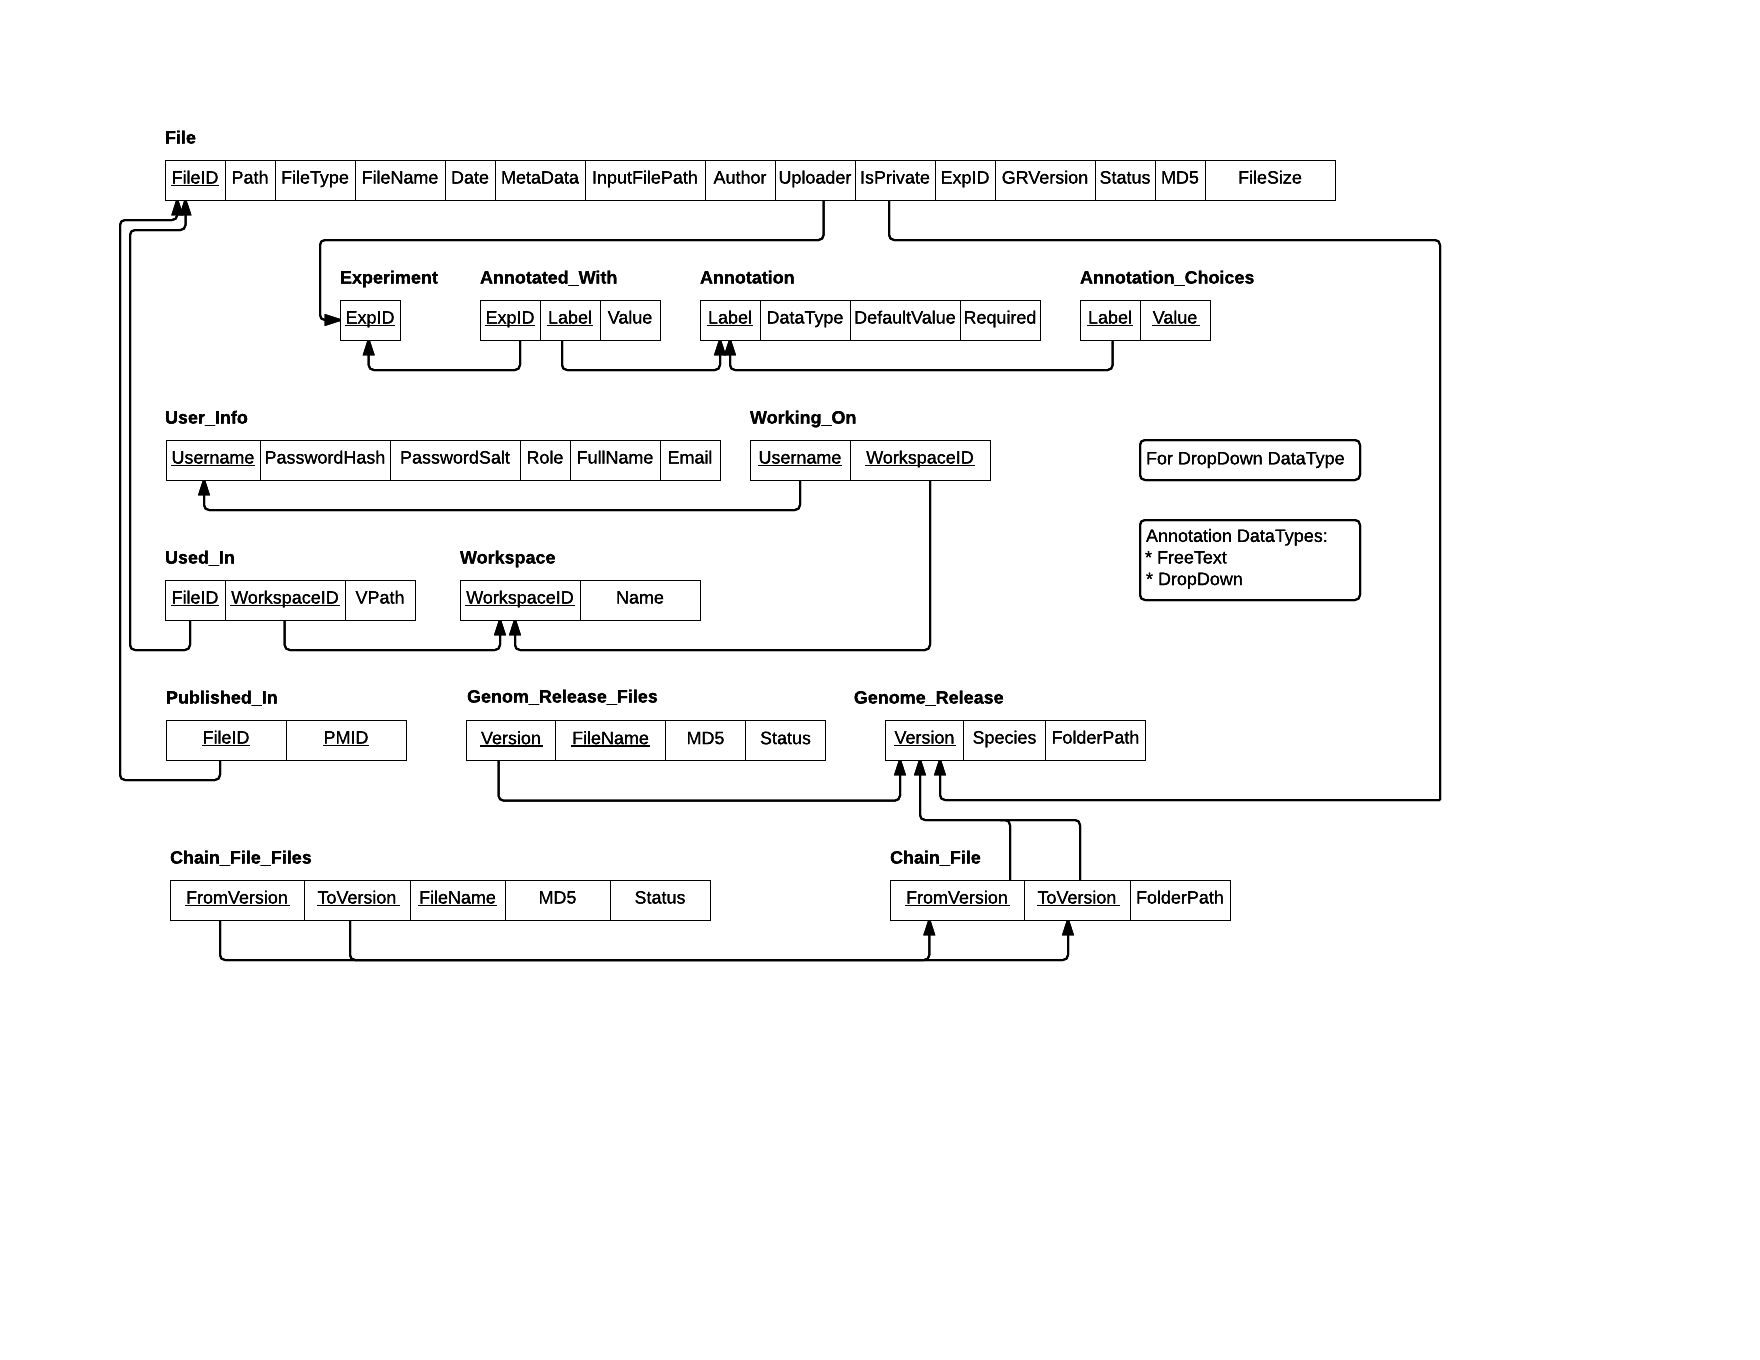
\includegraphics[width=20cm, angle=90, keepaspectratio=true]{dat_database_schema_v3.png}
%\addImageVertical{dat_database_schema_v3.png}
\caption{The database schema}
\label{fig:dat_databaseSchema}
\end{figure}

\FloatBarrier

\subsection{Database Design}
The following section will explain the less obvious columns and their intended use.

\texttt{FileID} is the identification number for a specific file. The data type \texttt{SERIAL} is used and will therefore be auto--generated by the database upon insertion.

\texttt{Path} is the path to the corresponding file in the file system, for example:
\texttt{/var/www/data/Experiment1/raw/rawFile1.fastq}

\texttt{MetaData} is the string of parameters used in processing and should be \texttt{NULL} for all raw files.

\texttt{Annotated\_With} is the table that enables the annotation of experiments, for example:
\begin{center}
  \begin{tabular}{| l | l | l |}
    \hline
    Experiment1 & Species & Dog \\
    \hline
  \end{tabular}
\end{center}

\texttt{Annotation} is the table containing all the possible annotations a user can use to provide extra information about an experiment. This includes the type of annotation which is \term{Drop Down} for annotations where the user can choose from a drop down list, or \term{Free Text} where the user can enter the value freely. There is also support for a default value and annotation forcing where users are forced to provide the information, for example:
\begin{center}
  \begin{tabular}{| l | l | l | l|}
    \hline
    Species & DropDown & Human & T \\ \hline
  \end{tabular}
\end{center}

\texttt{Annotation\_choices} is the table specifying the choices for \term{Drop Down} annotations, for example:\\
\begin{center}
  \begin{tabular}{| l | l | l | l|}
    \hline
    Species & Dog \\ \hline
    Species & Fly \\ \hline
  \end{tabular}
\end{center}

The \texttt{Genome\_Release} table stores information about the \term{Genome Releases} available for use. This includes the unique version code for a \term{Genome Release}\cite{UCSCGRVERSION}.

The \texttt{Genome\_Release\_Files} table stores the information about the files that make up the \term{Genome Release}.

\subsection{The Data Storage Subsystem}
All the classes used in the manipulation of the database and the creation of the file systems directory structure is contained in the java project's \texttt{database} package.

The other \appName\ subsystems execute all updates to the data storage through the \class{DatabaseAccessor} class. As a result there are many methods in this class, however most methods forwards the request to one of the classes in the \texttt{database.subclasses} package. Here the methods that modify the different areas of the data storage system are separated into different classes of more manageable sizes. An UML diagram of the \class{DatabaseAccessor} class and its subclasses is available in \refer{fig:dat_dbac} in  \refer{chap:dat_umls}.

The \class{DatabaseAccessor} utilizes a number of classes in order to return information to the method caller. These classes are contained in the \texttt{database.containers} package and are as follows:
\begin{itemize}
\item \class{Experiment}
\item \class{FileTuple}
\item \class{Annotation}
\item \class{Genome}
\end{itemize}

An UML diagram of these classes is also available in \refer{fig:dat_containers} in \refer{chap:dat_umls}.

\subsection{Interaction}
Below are examples of typical interactions with the \class{DatabaseAccessor} class.

\subsubsection{Adding an experiment}
In order to add an annotated experiment the following steps must be followed:
\begin{enumerate}
\item First the \term{addExperiment} method must be called. This will add one experiment to the database without any annotations set for that experiment. If you try to add one experiment that already exist then the addition will be refused and an exception will be thrown.

\item If there are no annotations that can be used to provide extra information about the experiment they must first be added by calling the \term{addFreeTextAnnotation} or \term{addDropDownAnnotation} methods.

\subitem If a \term{Drop Down} annotation already exists, but there is no suitable choice for the experiment a choice can be added by calling the \term{addDropDownAnnotationValue} method.

\item An available annotation can be used to provide extra information about an experiment by calling the \term{annotateExperiment} method.
\end{enumerate}

Now that an experiment has been added files can be added added to it.

\subsubsection{Annotation Handling}

Annotations can be handled using the methods below.

\begin{tabular}{|l| p{7cm}|}
\hline
\term{getChoices} & gets all the available annotation choices connected to a specific label. For example the possible choices returned for the label "sex" might be "Male, Female and Unknown". \\ \hline

\term{getAnnotations} & returns all annotation labels currently stored in the database. Examples could be "Sex,Species,Tissue,etc.". \\ \hline

\term{getAllAnnotationObjects} & Combines the two previous methods. Here an annotation object is returned that holds all the relevant information including the label, datatype, and the possible choices for a \term{Drop Down} annotation. \\ \hline

\term{changeAnnotationLabel} & updates the given label in the database. This will change the label for all experiments that use it. For example changing "specie" to "Species". \\ \hline

\term{changeAnnotationValue} & updates a value for a specific annotation label. For example changing "Human" to "Homosapien".  \\ \hline

\term{updateExperiment} & Updates an annotation for one specific experiment. Example: "experiment1, Species, Homosapien" can be changed to "experiment1, Species, Fly". \\ \hline

\term{deleteAnnotation} & deletes an unused annotation from the database. This will also delete all the choices for that annotation. \\ \hline

\term{removeAnnotationValue} & removes a single annotation value for a particular label. \\ \hline

\end{tabular}

\subsubsection{File Handling}
The actions of adding and deleting experiment files or genome releases can be performed using the following methods.

\begin{tabular}{|l| p{7cm}|}
\hline
\term{addNewFile} & To add a file you will need to have an experiment added before you call the \term{addNewFile} method. Raw files usually come in pairs and so they can be added together by specifying the input file name. \\ \hline

\term{deleteFile} & Deletes the given file from both the database and the file system. This can be done by either specifying the path or the file's ID number. \\ \hline

\term{addGenomeRelease} & Genome release files must be added one at a time by calling the \term{addGenomeRelease} method. This method returns an upload URL. \\ \hline

\term{removeGenomeRelease} & \term{removeGenomeRelease} removes all the files associated with a genome release. This can only be done if there are no files that have been generated using the specified genome release. \\ \hline
\end{tabular}